\documentclass[12pt,twoside]{article}
\usepackage[margin=0.5in]{geometry}
\usepackage[utf8]{inputenc}
\usepackage{setspace}
\usepackage{amsmath}
\usepackage{amsfonts}
\usepackage{amssymb}
\usepackage{enumerate}
\usepackage{tikz}
\usepackage{color}
\usepackage{natbib}
%\usepackage[superscript,biblabel]{cite}
\usepackage[unicode,hidelinks]{hyperref}

\renewcommand{\labelitemi}{$\bullet$}
\setstretch{1.1}
\setlength{\parskip}{0.4em plus0em minus0em}
\setcounter{secnumdepth}{0}
\setcounter{tocdepth}{2}
\def\NI{\noindent}
\def\NS{
	\setlength{\itemsep}{0.1em}
	\setlength{\parskip}{0em}
	\setlength{\parsep}{0em}
}
\def\RS{
	\setlength{\itemsep}{0em}
	\setlength{\parskip}{0.4em}
	\setlength{\parsep}{0em}
}

\begin{document}

\title{\textbf{Using structure to improve a noisy PPI network} \\ \Large{(now semi-coherent!)}}
\author{Douglas Myers-Turnbull\\ \texttt{dmyerstu@ucsd.edu}}
\date{\small{\today}}
\maketitle

\begin{abstract}
\NI \textbf{Motivation: } Protein-protein interaction (PPI) networks are often derived from noisy high-throughput experimental methods such as yeast two-hybrid screening. Consequently, PPI networks are typically both are cumbersome and suffer from low accuracy.\\
\NI \textbf{Methods: } Here we present a novel method (StructNA) for both reducing the size of PPI networks and improving their accuracy by finding homologs in the network whose interactions are consistent. Homologs are identified in a species-independent way using protein structural information. The method takes as input a single network. It identifies homologs, then merges fully homologous proteins and assigns scores to  interactions that are consistent among homologs. It considers both degree of homology and similarity of network topology for both the merging and scoring.\\
\NI \textbf{Results: } The method was able to correctly identify conserved interactions both across species and within individual species in benchmark sets derived from the Database of Interacting Proteins. On average, this resulted in a majority of interaction probabilities in the network being modified, and a reduction of network size between 5\% and 10\%. \\
\NI \textbf{Availability: } The algorithm was implemented in Java and is licensed under the Apache License version 2.0. It is freely available for download at \url{https://github.com/dmyersturnbull/network_merge}.
\end{abstract}

\section{Introduction}
\NI Protein-protein interaction (PPI) networks are often derived from high-throughput experimental assays such as Tandem affinity purification \cite{rigaut}, and yeast two-hybrid screening \cite{fields}. These techniques are used because they are cost-effective, but they frequently lead to the inclusion of false interactions and missing interactions, and they are unable to accurately determine the probability of interactions.

\NI PPI networks are modeled as undirected graphs in which vertices denote proteins and edges denote protein--protein interactions. Edge weights are used to describe the probability or certainty of an interaction. Psuedographs (which permit self-loops) allow for intramolecular interactions, and hypergraphs allow for multi-molecular interactions.

\NI A number of algorithms have been developed to decrease noise in PPIs by identifying homologs. These algorithms all solve a specific formulation of a \emph{network alignment problem}. The objective of this class of problems is, given two networks ($n$ networks in the case of a multiple network alignment), to define a mapping between vertices in the networks that maximizes their overlap. Here, ``overlap" can be given a number of definitions, but it usually incorperates both extent of homology between the aligned proteins and similarity of the network topology in the neighborhood of those proteins. Network alignment algorithms generally assume that homology is one-to-one in order to make the problem more tractable.

\NI There are a number of limitations inherent to these approaches. First, homology is not one-to-one in real biological systems. Consequently, network alignment algorithms fail to identify many homology relationships that are biological and should be used to inform interactions. Second, these algorithms cannot identify or use homology relationships between proteins within the same species. Finally, all current network alignment algorithms rely on sequence alignments to identify homologous pairs. Since the data describes physical interactions between proteins, sequence alignment is ill-suited for deciding homology.

\NI Therefore, we propose an algorithm for improving PPI networks that differs from network alignment algorithms in three ways:
\NS
\begin{enumerate}
\NS
\item It does not require that homology is one-to-one.
\item It can identify homology relationships within the same species.
\item It is based on structural information rather than sequence information, making it more suitable for use with PPIs.
\end{enumerate}

\NI The method uses the Structural Classification of Proteins (SCOP) \cite{scop} and structural alignment based on Combinatorial Extension \cite{ce} to introduce edges in the graph that indicate homology. It then uses this information to update the probability of interactions that are shared between homologous proteins. Finally, it collapses degenerate vertices via edge contraction, where degeneracy is decided by the presence of a clique whose members share interactions. Clique-finding is performed naively via the Bron--Kerbosch algorithm \cite{bron}, which was found to be sufficiently fast for biologically real networks.\RS

\subsection{Overview}

\NI We define two graphs: $(V, Int(G))$ and $(V, Hom(G))$, where the vertex set $V$ consists of proteins and is shared between both graphs, $(V, Int(G))$ is an interaction graph, and $(V, Hom(G))$ is a homology graph. Thus edges $e \in Int(G)$ denote interactions, and edges $e \in Hom(G)$ denote homology relations. The graph $G = (V,Int(G) \cup Hom(G))$ is a combined network consisting of both types of edges.

\NI Furthermore, for any $v \in Int(G)$, let $Int(v)$ be the set of neighbors of $v$ in $Int(G)$. We define $Hom(v)$ in the same way.

\NI The algorithm consists of three major steps.

\NI Given an interaction network $G=(V,Int(G))$, build a network $G'\,\! = (V,Int(G'\,\!) \cup Hom(G'\,\!))$ by using any available information (e.g. homology databases or alignment) to add edges to $Hom(G'\,\!)$ and to increase the weights of those edges. At the end of this process, remove any edge from $Hom(G'\,\!)$ with  weight less than some threshold $\tau$.

\NI For this process, we let $\alpha(a,b)$ denote the weighted score of an alignment that has been performed between vertices $a$ and $b$. Similarly, we let $\rho(a,b)$ denote the score of the most specific homology relation $r$ identified between nodes $a$ and $b$. For example, if $a$ and $b$ are from the same SCOP fold but not the same SCOP superfamily, $\rho(a,b)$ will be given by this relation.

\NI Second, generate a network $G'\,\!'\,\! = (V, Int(G'\,\!'\,\!)$ by using edges in $Hom(G'\,\!)$ to update edge weights (probabilities) in $Int(G)$. Use both the probability of the shared interaction and the probability of the homology for both interaction participants in this process.

\NI Remove any edge from $Hom(G'\,\!)$ with weight less than some threshold $\zeta$. Generate a network $G'\,\!'\,\!'\,\! = (V'\,\!, Int(G'\,\!'\,\!'\,\!) \cup Hom(G'\,\!'\,\!'\,\!))$ by merging nodes contained in cliques of $(V,Hom(G'\,\!'\,\!))$ in which every vertex in the clique is associated with the same set of neighbors  in $(V, Int(G'\,\!'\,\!))$.

\begin{figure}
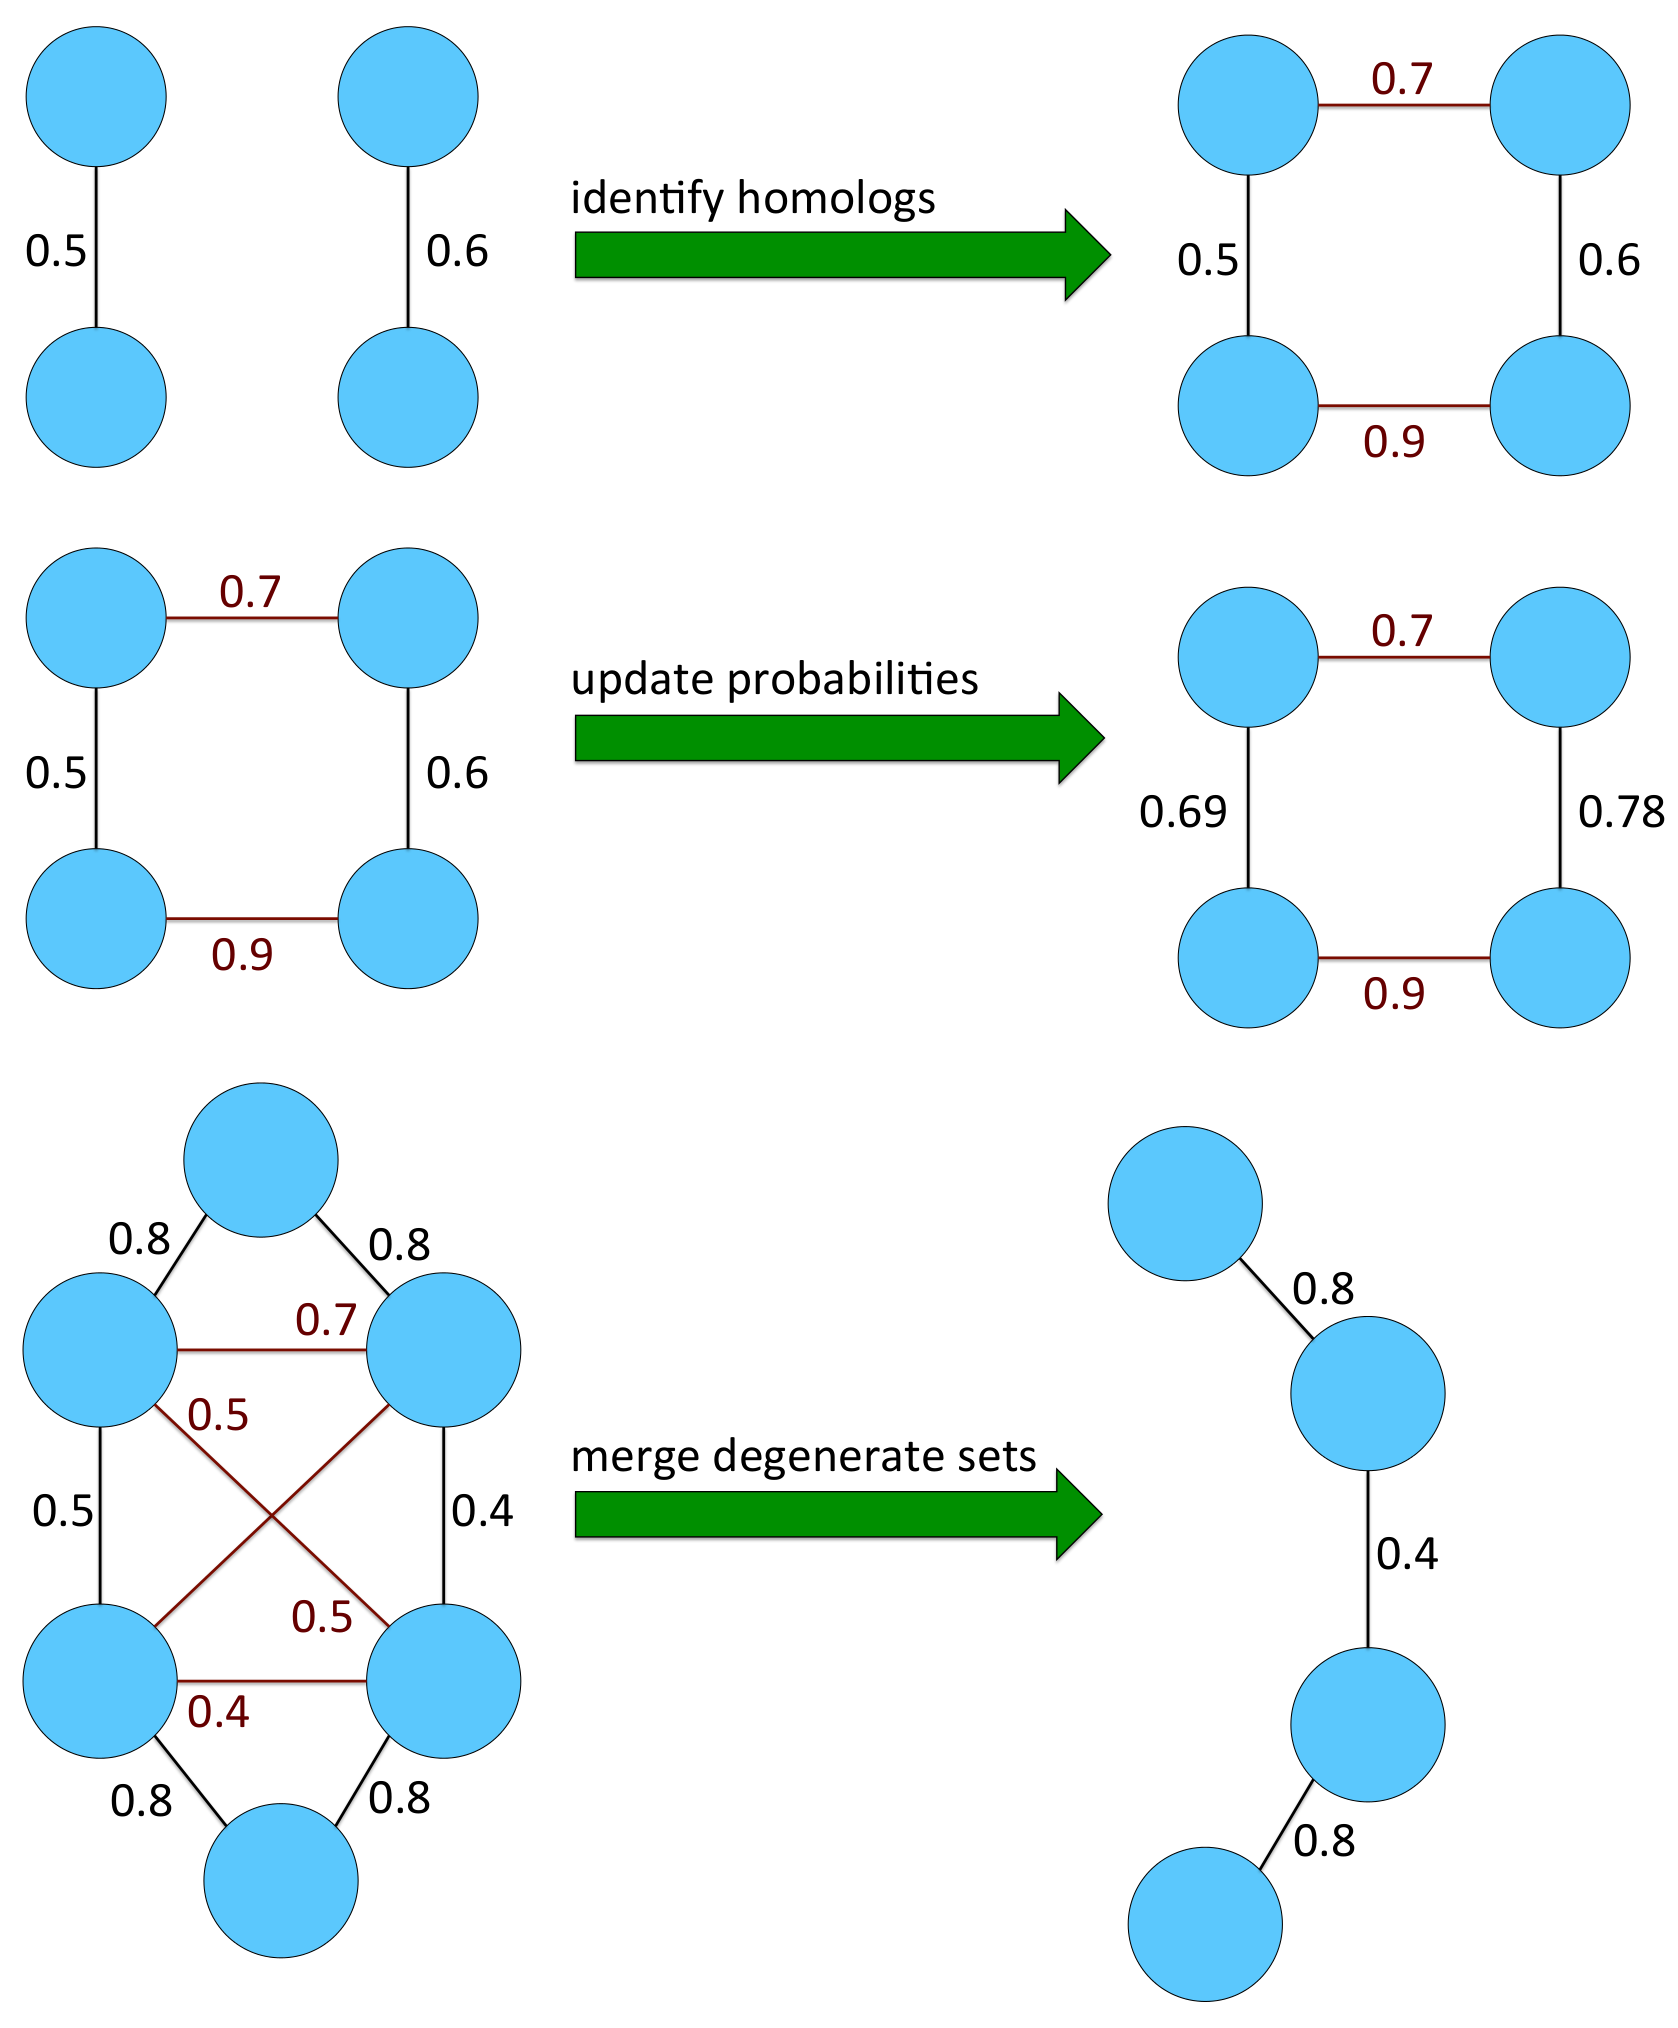
\includegraphics[scale=0.3]{three_steps.png}
\caption{The three major steps of StructNA. 1. Identify homologous pairs (red lines) using homolog databases and structural and sequences alignments. 2. Increase the probabilities of interactions that are conserved across homologs. 3. Merge vertices in cliques whose interactions are equivalent.}
\end{figure}

\subsection{Algorithm}

Given:
\vspace{-1em} \begin{itemize}\itemsep 0em
\item A graph $G=(V,Int(G) \cup Hom(G))$
\item Edge weights given by $Prob(e)$ for all $e \in Int(G)$
\item Edge weights given by $S(e)$ for all $e \in Hom(G)$
\item An homology scoring function $\Phi : V \times V \rightarrow [0,1]$, where $\Phi$ is a metric on $V$
\item A cutoff $\tau \in \mathbb{R}$
\item A cutoff $\zeta \in \mathbb{R}$, where $\zeta \geq \tau$
\item A depth parameter $\xi \in \mathbb{N}$
\end{itemize}
\NI StructNetAlign($G$, $\Phi$, $\tau$, $\zeta$, $\xi$):
\vspace{-0.5em} \begin{enumerate}
\NS
\item Parse network.
\item For every pair of vertices $(a,b)$, add an edge $(a,b)$ to $Hom(G)$, with label $ \Phi(a,b)$.
\item For every edge $e \in G$ such that $S(e) < \tau$, remove $e$.
\item For every edge $(u,v) \in Int(G)$:
\begin{enumerate}
\item Let $I=\emptyset$, and let $Q_a = 0, X_a = Y_a = 0 \; \forall \; a \in V$.
\item Run breadth-first search on $(V, Hom(G))$ from $u$ and $v$ concurrently to generate vertex labelings $X$ and $Y$, respectively. Stop after reaching depth $\xi$.
\item For both $R=X$ and $R=Y$, when visiting a vertex $b$ via edge $e$:
\begin{enumerate}
\item If $R_b=0$, let $R_b := 1$.
\item Let $Q := Q + \log S(e)$.
\item Let $R_b := R_b - exp(Q)$.
\end{enumerate}
\item For every edge $(x,y) \in Int(G)$ such $X_x \neq 0$ and $Y_y \neq 0$, let $Prob((u,v)) := Prob((u,v)) + 1 - X_x Y_y Prob((x,y))$.
\end{enumerate}
\item Discard every vertex $v$ such that $\iota(v) = 0$ and remove every edge incident to $v$.
\item For every edge $e \in G$ such that $S(e) < \zeta$, remove $e$.
\item Run the Bron--Kerbosch algorithm on $G_i$ to enumerate all maximal cliques $C = \{ c_1$ \ldots $c_x \}$, for clique sizes $\gamma(C_j) > 1 \; \forall j$.
\item Partition $C$ into sets $D = d_1 \ldots d_z$ such that $\forall \; v \in d_i, u \in d_j$, $Int(v) \neq Int(u)$, $\forall \; i,j$, and $Int(v) = Int(u) \; \forall u,v \in d_i \; \forall i$.
\item For each $d \in D$, merge by edge contraction every vertex in $d$, modifying the reference graph $G$.
\item Output the network $(V, Int(G))$.
\end{enumerate}

\subsection{Initial scoring of interactions}

\NI Interactions are given initial probabilities according to the number and type of experiment that identified them. In particular, we assign an interaction $X$ a probability of:

\NI $Prob(X) = \displaystyle Prob \left( \bigvee_{x \in X} x \right) = 1 - \prod_{x \in X} \left[1 - \kappa(x) Prob(x) \right]$,

\NI where each $x \in X$ is an experiment that determined interaction $X$, and $\kappa(x) \in [0,1]$ is the quality of the experiment that determined $x$. $\kappa$ ranged from $0.5$ for yeast two-hybrid to $1.0$ for protein complex co-immunoprecipitation, which is often considered a gold standard in protein--protein interaction detection \cite{kaboord}. The full listing for $\kappa$ is available as a supplemental (aka SFP).

\subsection{Establishing homology}
\NI In the first step, we identify homologs in the network. These are understood simply as proteins that are expected to have sufficient structural similarity to participate in some of the same chemistry and interact with other proteins in similar ways. In this way, homology is taken to be a species-independent property. A precise definition is decided by the alorithm based on the thresholds $\tau$ and $\zeta$. We deliberately conflate probability of homology and degree of homology. This is because our model is concerned with determined interactions that are conserved among homologs, which is probabalistic by nature. Thus we cannot reasonably discern between the two.
\NI A typical input network consists of a list interactions occurring between two polypeptide chains, where the chains are described by identifiers for UniProt \cite{uniprot}. In cases where the Protein Data Bank \cite{pdb} contains at least one structure for that chain, a PDB Id and is found for that UniProt Id. From that, a SCOP \cite{scop} domain corresponding to the PDB Id and chain are found. This selection process is problematic for multi-chain domains, for which we associate the chain with a domain arbitrarily.
\NI We rely on both alignment and information from third-party databases to establish homology. Structural information is preferred over sequence information where it is available. First, scores are assigned using SCOP by using the most specific SCOP relationship found. The particular scoring system was not chosen in a rigourous way but is listed below:

\begin{tabular}{lllll}
class & fold & superfamily & family & domain \\
$0.0$ & $0.1$ & $0.4$ & $0.8$ & $1.0$ \\
\end{tabular}

\NI In the case where a protein is not associated with a SCOP domain, the Pfam database is used instead. \RS
\NI In cases where homology is not established by SCOP \cite{scop} or Pfam relationships, homology can be derived either by structural alignment using Combinatorial Extension (CE) \cite{ce}, or by Needleman--Wunsch \cite{needleman} global sequence alignment. Structural alignment by Combinatorial Extension is preferred, so Needleman--Wunsch is only used in cases where a protein is not associated with a known structure in the Protein Data Bank \cite{pdb}.

\NI For CE, we use the scoring matrix SDM of Prlic et. al. \cite{prlic} added to BLOSUM62 \cite{blosum} with a coefficient of 2. We then score homology relationships using TM-Score \cite{zhang}, which is essentially an RMSD that is normalized by the protein length. A TM-score of $1.0$ is a perfect alignment, and a TM-score of $0.0$ has no aligned regions.

\NI For Needleman--Wunsch, we use BLOSUM62, a gap opening penalty of $-12$, and a gap extension penalty of $-1$. We then score homology relationships using percentage identity applied to a gamma distribution with shape $k=25.54$, scale $\theta=4.96$, and a linear shift of $0.2$, which was found by Weber et. al. \cite{webber} to give the best results for global alignment.

\subsection{Using homology to score interactions}

\NI The central idea here is very simple. Suppose we have four proteins $a$, $b$, $c$, and $d$ in the situtation shown in the figure. $a$ and $b$ interact, and $c$ and $d$ interact. Since $a$ is homologous to $c$ and $b$ is homologous to $d$, we now know with greater probability that $a$ and $b$ interact, and that $c$ and $d$ interact. (Indeed, we could also suggest that $a$ and $c$ interact.)

\NI We wish to use $y$ to increase $Prob(x)$. However, it would be inappropriate to let $x'\,\! := x \; \vee \; y$ and thereby $Prob(x)'\,\! := Prob(x) + Prob(y|\neg x)$, since this would not take into account the probabilities given by $\alpha$ and $\beta$. Instead, we let $x'\,\! := x \; \vee \; \alpha \beta y$ and thereby $Prob(x'\,\!) := Prob(x) + Prob(y | \neg x) Prob(\alpha) Prob(\beta)$. This way, we take into account both the probablity of an interaction and the probability that the interaction is homologous.

\NI We should favor being liberal when incorperating additional information into our model to alter probability. We can imagine a situtation in which $a$ has some interaction $x$, and $a$ is homologous to $b$ which is then homologous to $c$, but due to some limitation in our method or an underlying algorithm or database used in the above section, we do not have an edge from $a$ to $c$. If $c$ has some interaction $y$ that is similar to $x$, we would like to use $y$ to update the probability of $x$. This leads to the formulation below:

\NI Define
$R_{i,j}^{(u,v)} = Prob(i,j) \left(1 - \displaystyle Q_{u,i} - Q_{v,j} + Q_{u,i} \cdot Q_{v,j} \right)$

\NI Define $Q_{a,b} = \displaystyle \prod_{\text{paths } \pi \text{ from a to b}} \left( 1 - \prod_{k} S(\pi_k) \right)$

\NI Then we want to update the probability of an interaction $(u,v)$ with:

\NI $Prob((u,v))'\,\! = Prob((u,v)) + 1 - \displaystyle \prod_{i,j}(1 - R_{i,j}^{(u,v)})$

\NI Unfortunately, this would require use to enumerate all possible paths. Therefore, we need to be satisfied with the assumption that our homology graph contains every edge that it should. Under this assumption, a case like the one described above is a violation of the idea of homology, since homology should be a metric on our graph and thus obey the triangle inequality. With this in mind, we approximate the above by taking only the shortest path rather than all paths. This simplifies the definition of $Prob((u,v))$ to:

\NI $Prob((u,v))'\,\! = Prob((u,v)) + \displaystyle Prob((i,j)) \left( \prod_{\pi_k \in \pi^i}(S(\pi_k^i) \prod_{\pi_k \in \pi^j}(S(\pi_k^j) - Prob((x,y)) \prod_{\pi_k \in \pi^i}(S(\pi_k^i) \prod_{\pi_k \in \pi^j}(S(\pi_k^j) \right)$,

\NI where $(i,j)$ is the closest interaction corresponding to $(u,v)$, and $\pi^i, \pi^j$ are the shortest paths corresponding to $u \ldots i$ and $v \ldots j$, respectively.

\subsection{Merging degenerate vertex sets}

\NI Unfortunately, \textsc{Max-Clique} is \textsc{NP-Equivalent} and \textsc{APX-Hard}. The best known polynomial-time approximation algorithm has an error bound of $\epsilon = \mathcal O \left(\frac{n}{\log^2(n)}\right)$ \cite{boppana}. This makes even approximating a solution to \textsc{Max-Clique} intractable according to worst-case time-complexity. However, \textsc{Max-Clique} is often solvable in practice for small $n$ because, unlike many other \textsc{NP-Hard} problems, naive algorithms for \textsc{Max-Clique} do not require numerically intensive steps. The Bron--Kerbosch algorithm requires only incrementation and trivial set unions and subtractions. Consequentially, it has been found to perform well enough in practice for reasonable $n$ such as those found in real biological networks.

\NI Moreover, we can bound the time-complexity of a naive algorithm (such as Bron--Kerbosch) in terms of the maximum number of homology edges of any vertex in $G$.

\NI Let $\iota(v)$ denote the number of edges $(v, v'\,\!)$ in $Int(G)$, $\forall \: v \in V$, and let $\eta(v)$ denote the number of edges $(v, v'\,\!)$ in $Hom(G)$, $\forall \: v \in V$. Let $\iota^* = \displaystyle \max_{v \in V}\{\iota(v)\}$, $\eta^* = \displaystyle \max_{v \in V}\{\eta(v)\}$.

\NI Let $\gamma$ be the maximal clique size in $Hom(G)$. Then $\gamma^* \leq \eta^*$.\\
\NI We can readily solve \textsc{Max-Clique}$(G)$ in $\mathcal O(|V|^{\eta^*}(\eta^*)^3)$ time by enumerating all $|V|^{\gamma}$ subgraphs of size $\gamma$ for every $\gamma = 1, 2, \ldots, \eta^*$.

\NI Our goal is to identify degenerate sets of vertices. To do this, we require subgraphs with edges in $Int(G'\,\!)$, and homology relations between the two subgraphs that result in a clique in $(V,Hom(G)$. A subset of $Hom(G'\,\!'\,\!)$ defines an isomorphism between two subgraphs of $(V'\,\!, Int(G'\,\!'\,\!))$.

\NI Given a clique $C$, we need to find which vertices in $C$ share interactions. This results in a partitioning of $C$ into disjoint induced subgraphs $D$. We can then merge every vertex in each $D_i$.

\NI We call a subset $S \subseteq C$ for some clique $C \in (V,Hom(G'\,\!))$ degenerate if $\forall u,v \in S \; Int(u) = Int(v)$. If $C$ is a maximal clique and $\not \exists S_1 \subseteq C, \; S_1 \supset S$ for some degenerate set $S_1$, we say $S$ is a \emph{maximal} degenerate set.

\NI We first identify all maximal cliques on $(V,Hom(G'\,\!))$ using the {Max-Clique} algorithm by Bron and Kerbosch \cite{bron}, which has been found in practice to be faster than algorithms with superior worst-case time complexity. We then identify maximal degenerate sets by associating to each vertex of a clique $C$ a string that uniquely identifies its interactions, then partitioning $C$.

\NI If a vertex $v \in V$ belongs to two distinct maximal degenerate sets $S_1$ and $S_2$, we choose whether to include $v$ in $S_1$ or $S_2$ by the following:
\vspace{-1.5em} \begin{enumerate}[i)]
\item If $|S_1| > |S_2|$, choose $S_1$
\vspace{-1.5em} \item If $|S_1| = |S_2|$, choose the set whose sorted vertex labels form the lexicographically smaller string
\vspace{-1.5em}\end{enumerate}

\NI Finally, we perform edge contraction on each degenerate set with respect to both $(V,Int(G'\,\!))$ and $(V,Hom(G'\,\!))$. The vertex $v_0$ with the lexicographically smallest label for each degenerate set is chosen as the representative, and the labels of the other vertices are included as metadata in $v_0$.

\subsection{Implementation}

\NI The method was implemented in Java, using many standard Java 7 features. It is clearly documented and is under 6,000 SLOC. It is distributed under the Apache License version 2. A distribution is available for download at \url{https://github.com/dmyersturnbull/network_merge}.

\section{Results}

\NI 

\subsection{Overview}

\subsection{Accuracy}

\subsection{Speed}

\NI The method was implemented in Java and run on a JDK 7 platform on a single AMD Phenom II processor with 4GB of DDR3 memory. In general, the most time-consuming step was pairwise alignment in cases where a cached alignment result was unavailable. The second and third steps were found to require less than an hour for even extremely large networks of hundreds of thousands of proteins.

\section{Appendix 1. Formal proofs}

\bibliographystyle{plain}
\bibliography{citations}

\end{document}